% ============================================================================
% 动态第三方风险（TPR）精细化量化模型 - 04_dynamic_tpr_models.tex
% ============================================================================

\section{动态第三方风险（TPR）模型}
\label{sec:tpr_models}
在这一节，我们采用风险因子动态缩放坠机概率基础常数的方法来建立时空坠机概率模型，并将其应用到致命风险成本、财产损失风险成本以及噪声滋扰社会影响成本的动态评估中.
% ============================================================================
% 基础坠机概率模型
% ============================================================================
\subsection{复杂微气象与建筑耦合的动态坠机概率评估}
\label{subsec:pcrash_model}
无人机坠机是小概率事件，在不同的环境因素影响下，坠机概率会发生显著变化。为了更准确地评估坠机风险，我们引入了风场因子、降雨因子和建筑因子等动态环境因素，通过以下模型来动态调整基础坠机概率。

借鉴Cox比例风险模型（Proportional Hazards Model, PHM）的框架，我们将基准风险率与环境协变量的乘积形式应用于无人机坠机概率建模。定义综合缩放因子$\Phi(x,y,z,t)$为各环境因子的乘积：

\begin{equation}
\Phi(x,y,z,t) = f_{wind}(x,y,z,t) \cdot f_{rain}(x,y,t) \cdot f_{obs}(x,y,z)
\label{eq:phi_composite}
\end{equation}

其中$f_{wind}$、$f_{rain}$和$f_{obs}$分别代表风场因子、降雨因子和城市建筑因子，各因子的具体定义将在后续小节中给出。基于此综合缩放因子，时空动态坠机概率$P_{crash}(x,y,z,t)$采用指数截断形式：

\begin{equation}
P_{crash}(x,y,z,t) = 1 - \exp\bigl( -\lambda_{base} \cdot \Phi(x,y,z,t) \cdot \Delta t \bigr)
\label{eq:pcrash_dynamic}
\end{equation}

其中$\lambda_{base}$为无人机在晴朗空旷无风环境下的基准失效率（经验常数），$\Delta t$为无人机通过当前航段的飞行时间。该指数形式保证了$P_{crash} \in [0,1)$，避免概率溢出；当$\lambda_{base} \cdot \Phi \cdot \Delta t \ll 1$时，可近似为$P_{crash} \approx \lambda_{base} \cdot \Phi \cdot \Delta t$，退化为线性形式。下面分别定义各动态缩放因子。
% ============================================================================
% （风场因子）
% ============================================================================
\subsubsection[Wind Field Factor]{风场因子}
\label{subsubsec:f_wind}
风速对无人机的影响呈现非线性指数特征，在抗风极限以下, 控制难度
随风速增加而急剧上升; 超过抗风极限后, 失控概率趋于无穷大。因此，我们定义风场因子$f_{wind}$如下：

\begin{equation}
f_{wind}(x,y,z,t) = 
\begin{cases} 
e^{k_w \cdot \left( \dfrac{v_{wind}}{V_{limit}} \right)^\theta}, & v_{wind} < V_{limit} \\
+\infty, & v_{wind} \ge V_{limit} 
\end{cases}
\label{eq:f_wind}
\end{equation}

\begin{figure}[htbp]
    \centering
    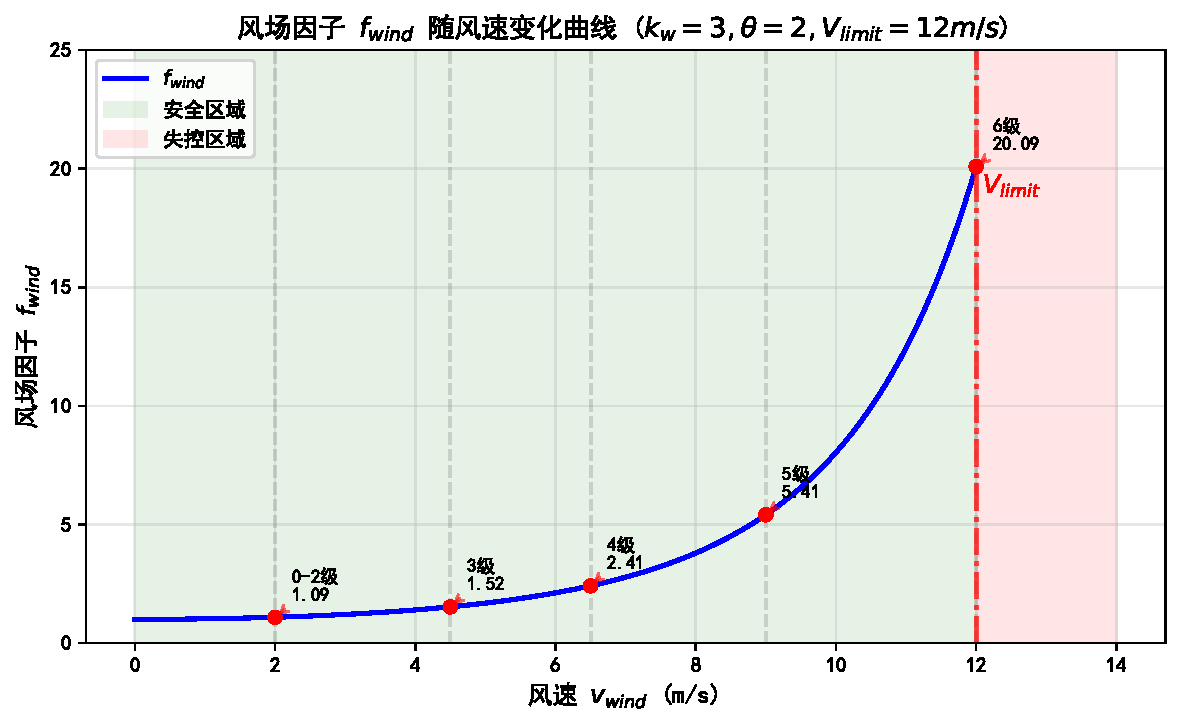
\includegraphics[width=0.8\linewidth]{figures/f_wind_curve.pdf}
    \caption{风场因子随风速变化曲线}
    \label{fig:f_wind_curve}
\end{figure}

\begin{table}[htbp]
\centering
\caption{风场因子边界条件验证($k_w=3, \theta=2$)}
\label{tab:wind_speed}
\renewcommand{\arraystretch}{1.3}
\begin{tabular}{c c c c}
\toprule
\textbf{蒲福风级} & \textbf{典型风速 $v$ (m/s)} & \textbf{无量纲比 $v/V_{\text{limit}}$} & \textbf{$f_{\text{wind}}$} \\
\midrule
0--2 级 & 2.0 & 0.17 & 1.09 \\
3 级    & 4.5 & 0.38 & 1.54 \\
4 级    & 6.5 & 0.54 & 2.40 \\
5 级    & 9.0 & 0.75 & 5.40 \\
6 级    & 12.0 & 1.00 & 20.09 \\
$\geq$ 7 级 & $>12.0$ & $>1.00$ & $+\infty$\\
\bottomrule
\end{tabular}
\end{table}

% ============================================================================
% （降雨因子）
% ============================================================================

\subsubsection[Rainfall Factor]{降雨因子}
\label{subsubsec:f_rain}
降雨对无人机飞行的影响主要体现在增加空气阻力、降低能见度以及引起设备故障等方面。为了量化降雨对坠机概率的影响，我们定义降雨因子$f_{rain}$如下：

\begin{equation}
f_{rain}(x,y,t) = 1 + \gamma \cdot I_{rain}(x,y,t)^2
\label{eq:f_rain}
\end{equation}

\begin{figure}[ht]
    \centering
    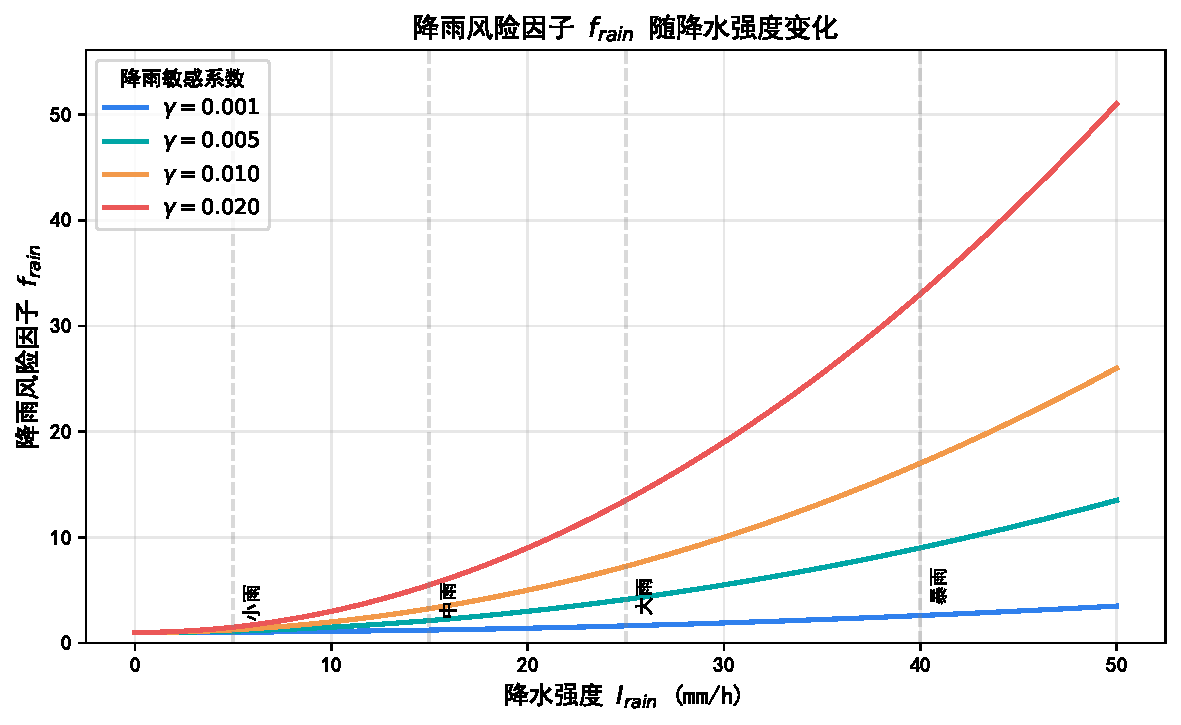
\includegraphics[width=0.8\linewidth]{figures/f_rain_curve.pdf}
    \caption{降雨因子随降雨强度变化曲线}
    \label{fig:f_rain_curve}
\end{figure}

\begin{table}[ht]
\centering
\caption{降雨因子边界条件验证($\gamma=0.005$)}
\label{tab:rainfall}
\renewcommand{\arraystretch}{1.3}
\begin{tabular}{l c c}
\toprule
\textbf{降雨强度级别} & \textbf{小时雨强 $I$ (mm/h)} & \textbf{$f_{\text{rain}}$} \\
\midrule
无雨             & 0.0  & 1.00 \\
小雨             & 2.0  & 1.02 \\
中雨             & 6.0  & 1.18 \\
大雨             & 12.0 & 1.72 \\
暴雨             & 25.0 & 4.13 \\
极端降水         & 50.0 & 13.50 \\
\bottomrule
\end{tabular}
\end{table}


% ============================================================================
% （建筑因子）
% ============================================================================
\subsubsection[Static Urban Building Factor]{建筑因子}
\label{subsubsec:f_obs}
城市建筑对无人机飞行安全的影响主要来源于天空可视度受限、建筑物高度遮挡以及建筑密度导致的导航复杂度。为了量化城市建筑对坠机概率的影响，我们定义城市建筑因子$f_{obs}$如下：

\begin{equation}
f_{obs}(x,y,z) = 1 + K_{obs} \cdot R_{canyon}(x,y,z)
\label{eq:f_obs}
\end{equation}

其中$K_{obs}$为环境敏感度放大系数（典型取值 10），$R_{canyon}(x,y,z)$为基于高度分层的城市峡谷综合干扰指数，反映了城市峡谷的复杂程度和建筑物的密集程度。它由以下三个部分组成：

\begin{equation}
R_{canyon}(x,y,z) = w_1 [1 - \text{SVF}(x,y,z)]^\alpha + w_2 \frac{H_{avg}(x,y)}{z + \epsilon} + w_3 D_{building}(x,y)
\label{eq:r_canyon}
\end{equation}

其中$w_1, w_2, w_3$是权重系数，$\text{SVF}(x,y,z)$为天空可视因子，反映天空被建筑物遮挡的程度；$H_{avg}(x,y)$为周围建筑物的平均高度；$D_{building}(x,y)$为建筑密度指标，反映单位面积内的建筑分布密集程度。各项的物理机制严格映射了无人机在不同飞行高度下的风险受迫程度

\begin{table}[htbp]
\centering
\caption{城市建筑因子边界条件验证($K_{obs}=10$)}
\label{tab:urban_validation}
\renewcommand{\arraystretch}{1.3}
\begin{tabular}{l c c}
\toprule
\textbf{城市场景} & \textbf{$R_{canyon}$} & \textbf{$f_{obs}$} \\
\midrule
开阔地   & 0   & 1.00 \\
低密度区 & 0.2 & 3.00 \\
中密度区 & 0.5 & 6.00 \\
高密度区 & 0.8 & 9.00 \\
城市峡谷 & 1.0 & 11.00 \\
\bottomrule
\end{tabular}
\end{table}

无人机飞行在晴朗无风的开阔地带时，模型自洽退化为$P_{crash} = 1 - \exp(-\lambda_{base} \cdot \Delta t) \approx \lambda_{base} \cdot \Delta t$。

% ============================================================================
% 致命风险成本和财产损失风险成本
% ============================================================================
\subsection{致命风险成本和财产损失风险成本}

\subsubsection{致命风险成本}

致命风险成本（Fatality risk cost）定义为无人机坠毁导致地面行人和车辆内人员伤亡的期望成本，其单位为每飞行小时的死亡人数。总致命风险成本记为 $c_{\mathrm{rf}}$，它由针对行人的致命风险成本 $c_{\mathrm{rp}}$ 以及针对车辆内人员的致命风险成本 $c_{\mathrm{rv}}$ 两部分组成：

\begin{equation}
c_{\mathrm{rf}} = c_{\mathrm{rp}} + c_{\mathrm{rv}}
\label{eq:fatality_risk_total}
\end{equation}

\paragraph{行人致命风险}
无人机在飞行过程中可能因失去控制而坠落并撞击地面行人。评估行人致命风险成本通常需要考虑三个级联过程：(1) 无人机系统发生故障失效；(2) 失控无人机坠落并撞击地面行人；(3) 撞击动能对行人造成致命性伤害。这一连串动作共同决定了最终的风险暴露水平。行人致命风险成本 $c_{\mathrm{rp}}$ 定义为每飞行小时的预期死亡人数，计算公式如下：

\begin{equation}
c_{\mathrm{rp}} = P_{\mathrm{crash}} N_{\mathrm{hit}}^p R_{\mathrm{f}}^p
\label{eq:pedestrian_fatality}
\end{equation}

其中，$P_{\mathrm{crash}}$ 为无人机系统失效概率，主要取决于硬件可靠性与飞行环境的复杂程度；$N_{\mathrm{hit}}^p$ 为坠机覆盖区域内的预期受击行人数（与人口密度高度相关）；$R_{\mathrm{f}}^p$ 为行人在遭受撞击后的致死率。在公式 \eqref{eq:pedestrian_fatality} 中，变量 $N_{\mathrm{hit}}^p$ 与人口密度相关，定义为：

\begin{equation}
N_{\mathrm{hit}}^p = S_{\mathrm{hit}} \cdot \rho_{\mathrm{pop}}(x,y,t)
\label{eq:pedestrian_hit_count}
\end{equation}

撞击致死率 $R_{\mathrm{f}}^p$ 与无人机的重量和下落高度相关。为保证模型满足基本物理单调性，即撞击动能增大时致死率不应下降，本文采用基于撞击动能的致死率函数：

\begin{equation}
R_{\mathrm{f}}^p =
\frac{1}{1 + \sqrt{\frac{\alpha}{\beta}}
\left(\frac{\beta}{E_{\mathrm{imp}}}\right)^{\frac{1}{4S_c}}}
\label{eq:fatality_rate}
\end{equation}

其中，$\alpha$ 与 $\beta$ 为致死率模型参数，$S_c$ 为行人遮蔽系数，$E_{\mathrm{imp}}$ 为无人机撞击地面时的动能。由式 \eqref{eq:fatality_rate} 可知，当 $E_{\mathrm{imp}}\rightarrow\infty$ 时，$R_{\mathrm{f}}^p\rightarrow1$；当 $E_{\mathrm{imp}}\rightarrow0$ 时，$R_{\mathrm{f}}^p\rightarrow0$，因此该形式与撞击伤害的物理直觉一致。撞击动能计算如下：

\begin{equation}
E_{\mathrm{imp}} = \frac{1}{2} m v^2
\label{eq:impact_energy}
\end{equation}

考虑到空气阻力的影响，坠落过程中的空气阻力 $F_d$ 可表示为：

\begin{equation}
F_d = \frac{1}{2} R_I \rho_A S_{\mathrm{ref}} v^2
\label{eq:drag_force}
\end{equation}

其中，$R_I$ 为空气阻力系数，$\rho_A$ 为空气密度，$S_{\mathrm{ref}}$ 为无人机下落过程中的气动参考面积。需要注意的是，$S_{\mathrm{ref}}$ 与式 \eqref{eq:pedestrian_hit_count} 中的坠机覆盖面积 $S_{\mathrm{hit}}$ 具有不同物理含义：前者描述无人机迎风阻力面积，后者描述地面暴露目标可能被击中的等效面积。若缺乏无人机详细几何参数，可在实验中采用简化假设 $S_{\mathrm{ref}}\approx S_{\mathrm{hit}}$，但二者在模型定义上应保持区分。

取竖直向下方向为正，则无人机坠落的瞬时加速度 $a$ 为：

\begin{equation}
a = \frac{F_g - F_d}{m}
= g - \frac{R_I \rho_A S_{\mathrm{ref}} v^2}{2m}
\label{eq:acceleration}
\end{equation}

由于目标是求无人机从高度 $h$ 坠落至地面时的撞击速度，应将加速度写为高度的函数。利用链式法则 $a=\frac{dv}{dt}=v\frac{dv}{dh}$，并令 $k=\frac{R_I \rho_A S_{\mathrm{ref}}}{2m}$，有：

\begin{equation}
v\frac{dv}{dh} = g - k v^2
\label{eq:velocity_height_ode}
\end{equation}

对下落高度进行分离变量积分：

\begin{equation}
\int_{0}^{v(h)} \frac{v'}{g-kv'^2}\,dv'
= \int_{0}^{h} dh'
\label{eq:impact_velocity_integral}
\end{equation}

解得无人机自高度 $h$ 坠落后的撞击速度为：

\begin{equation}
v(h) =
\sqrt{\frac{2mg}{R_I \rho_A S_{\mathrm{ref}}}
\left(1 - e^{-\frac{h R_I \rho_A S_{\mathrm{ref}}}{m}}\right)}
\label{eq:impact_velocity}
\end{equation}

\paragraph{车辆人员致命风险}
类似地，对于行驶在道路上的车辆，其内部人员的致命风险成本 $c_{\mathrm{rv}}$ 同样取决于系统失效概率、受击车辆数以及车辆防护下的致死率：

\begin{equation}
c_{\mathrm{rv}} = P_{\mathrm{crash}} N_{\mathrm{hit}}^v R_{\mathrm{f}}^v
\label{eq:vehicle_fatality}
\end{equation}

其中，$N_{\mathrm{hit}}^v$ 为预期受击车辆数，与实时交通流密度相关：

\begin{equation}
N_{\mathrm{hit}}^v = S_{\mathrm{hit}} \cdot \rho_{\mathrm{veh}}(x,y,t)
\label{eq:vehicle_hit_count}
\end{equation}

车辆外壳和车顶结构会显著削弱小型无人机撞击对车内人员的直接伤害，因此车辆人员致死率不宜直接等同于行人致死率。考虑到车辆内部人员伤亡往往受车辆结构、撞击位置和交通事故场景共同影响，本文采用统计平均致死率对 $R_{\mathrm{f}}^v$ 进行估计。具体而言，$R_{\mathrm{f}}^v$ 表示车辆事故中车内人员死亡的平均概率，可由研究区域内年度交通事故统计数据得到：

\begin{equation}
R_{\mathrm{f}}^v =
\frac{N_{\mathrm{fatal}}^{\mathrm{veh}}}{N_{\mathrm{acc}}^{\mathrm{veh}}}
\label{eq:vehicle_fatality_rate}
\end{equation}

其中，$N_{\mathrm{fatal}}^{\mathrm{veh}}$ 为年度交通事故导致的车内人员死亡总数，$N_{\mathrm{acc}}^{\mathrm{veh}}$ 为同一统计口径下的年度交通事故总数。若研究区域缺乏细粒度交通事故数据，可采用城市或国家层面的公开统计年鉴作为近似，并在敏感性分析中检验该参数对路径结果的影响。

在计算上述致命风险时，地表暴露的易损目标（行人和车辆）密度是随时间动态波动的。设 $\rho_{\mathrm{pop}}(x,y,t)$ 与 $\rho_{\mathrm{veh}}(x,y,t)$ 分别为时空坐标 $(x,y,t)$ 处的动态人口密度与车辆密度。这两个时空场分布矩阵将作为外部已知先验数据（Prior Data）输入至评估模型中。
该定义方式展现了评估模型的通用性，即只要输入相应的时空密度数据，模型即可实现对不同环境下的动态风险评估。详细的动态密度矩阵数学生成过程参见附录 \ref{appendix:poi_model}。

% ============================================================================
% （财产损失风险成本）
% ============================================================================

\subsubsection{财产损失风险成本}

本文将财产损失风险成本定义为无人机在低空飞行或失控坠落过程中对建筑物造成的潜在影响。与行人和车辆风险不同，建筑物作为静态地物，其风险暴露主要取决于建筑高度、建筑横截面积以及无人机当前飞行高度之间的空间关系。在复杂城市空地环境中，建筑高度通常呈现右偏长尾分布，高层建筑数量随高度增加而快速减少，因而可采用对数正态分布对建筑高度进行刻画。设研究区域内第 $k$ 栋建筑的高度为 $h_{\mathrm{b}}^k$，建筑总数为 $N_{\mathrm{total}}$，则建筑高度对数值的均值 $\mu$ 与标准差 $\sigma$ 定义为：

\begin{equation}
\mu = \frac{1}{N_{\mathrm{total}}}
\sum_{k=1}^{N_{\mathrm{total}}} \ln h_{\mathrm{b}}^k
\label{eq:building_height_mean}
\end{equation}
\begin{equation}
\sigma =
\sqrt{
\frac{1}{N_{\mathrm{total}} - 1}
\sum_{k=1}^{N_{\mathrm{total}}}
\left(\ln h_{\mathrm{b}}^k - \mu\right)^2
}
\label{eq:building_height_std}
\end{equation}

在给定无人机飞行高度 $h$ 时，第 $k$ 栋建筑对无人机造成的单位财产风险强度记为 $r_{\mathrm{b}}^k(h)$。考虑到高度低于阈值 $e^\mu$ 的建筑在城市中分布较为密集，其风险强度主要随高度以 $1/h$ 的形式衰减；而当建筑高度超过 $e^\mu$ 后，高层建筑数量随高度增加呈指数式下降，因此引入对数正态尾部项刻画稀有高层建筑的衰减效应：

\begin{equation}
r_{\mathrm{b}}^k(h) =
\begin{cases}
\dfrac{1}{h\sigma\sqrt{2\pi}}, & 0 < \ln h \leq \mu, \\[6pt]
\dfrac{1}{h\sigma\sqrt{2\pi}}
\exp\left[-\dfrac{(\ln h - \mu)^2}{2\sigma^2}\right], & \ln h > \mu.
\end{cases}
\label{eq:single_building_risk}
\end{equation}

进一步地，设空间单元 $i$ 内共有 $N_i$ 栋建筑，第 $k$ 栋建筑的平面横截面积为 $S_{\mathrm{b}}^k$。由于建筑物作为障碍物只有在无人机飞行高度不高于其自身高度时才会干扰飞行或产生潜在碰撞损失，因此引入指示函数 $\mathbb{I}\{h \leq h_{\mathrm{b}}^k\}$。单元 $i$ 在高度 $h$ 下的总体财产风险成本可表示为：

\begin{equation}
r_{\mathrm{b}}^i(h) =
\sum_{k=1}^{N_i}
\left[
r_{\mathrm{b}}^k(h)
\cdot S_{\mathrm{b}}^k
\cdot \mathbb{I}\{h \leq h_{\mathrm{b}}^k\}
\right]
\label{eq:unit_property_risk}
\end{equation}

式 \eqref{eq:unit_property_risk} 同时考虑了建筑高度和建筑密度两个因素：高度项决定建筑是否会在当前飞行高度上构成障碍，横截面积项则用于区分建筑密集单元与建筑稀疏单元的暴露强度。由此得到的 $r_{\mathrm{b}}^i(h)$ 可作为后续路径规划中财产损失风险张量 $R_{\mathrm{property}}(x,y,z)$ 的静态空间分量，并可通过时间维广播与动态坠机概率 $P_{\mathrm{crash}}(x,y,z,t)$ 结合，形成时空财产损失期望成本。

\subsection{噪声滋扰社会影响成本}

噪声在无人机飞行过程中不断产生，且其对地表环境的影响在时间与空间维度上均呈现出显著的动态波动性。

\begin{figure}[htbp]
    \centering
    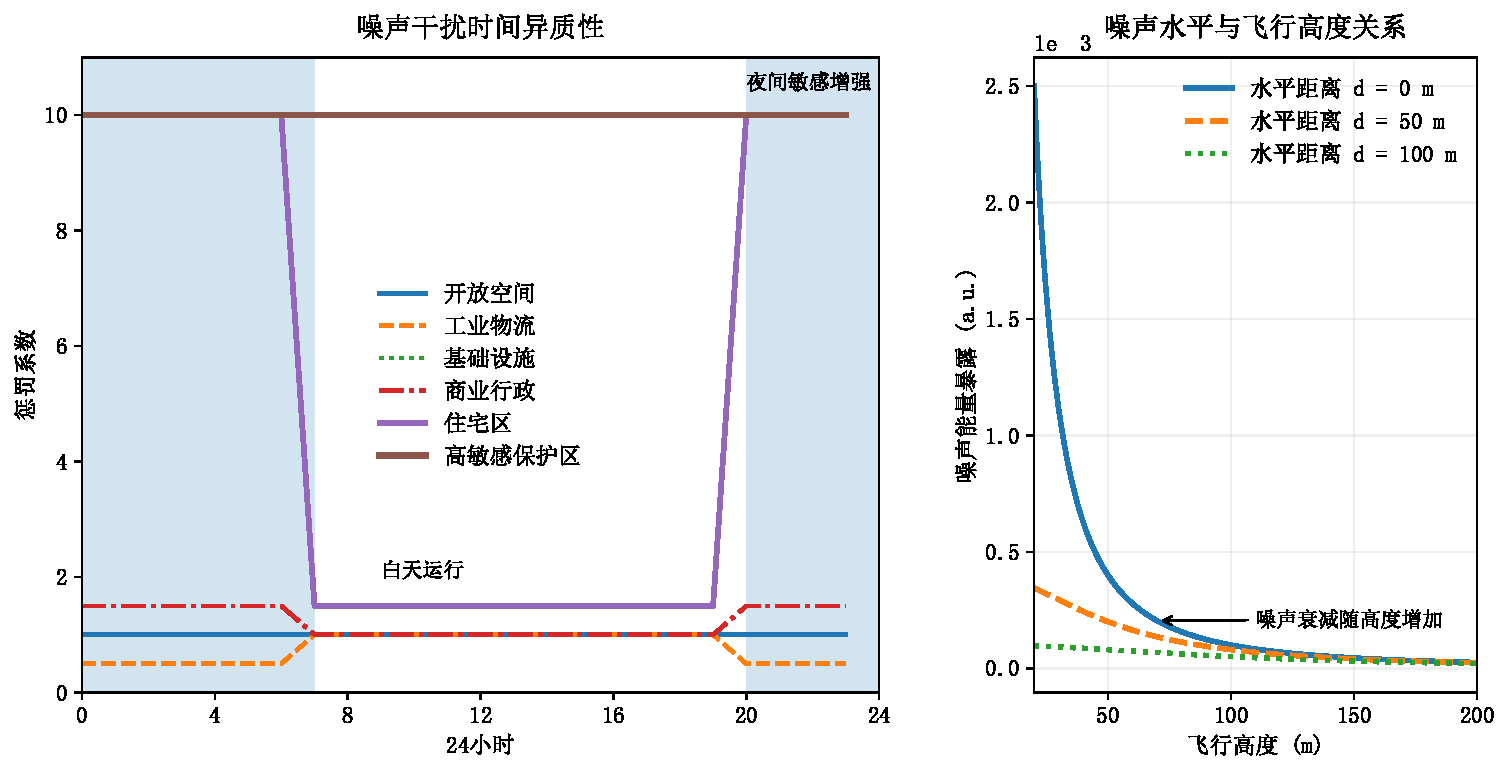
\includegraphics[width=0.8\textwidth]{figures/noise_temporal_matrix.pdf}
    \caption{噪声对环境影响}
    \label{fig:noise_temporal_matrix}
\end{figure}

为了在三维轨迹优化中能够可计算地定量评估噪声扰民的时空差异，并避免对数尺度（如分贝）在路径全局积分中带来的非线性病态问题，本文从声学能量守恒定律出发，定义噪声成本为地表受体单元接收到的“等效噪声能量暴露”与受影响社会人口期望的乘积：

\begin{equation}
Cost_{\mathrm{noise}}(i, t) = E_{\mathrm{noise}}(i, t) \times \rho_{\mathrm{pop}}(i, t) \times S_{\mathrm{landuse}}(i) \times T_{\mathrm{penalty}}(t)
\label{eq:noise_cost}
\end{equation}

其中，$E_{\mathrm{noise}}(i, t)$ 表示时刻 $t$ 无人机在地面网格单元 $i$ 处产生的人均“地表噪声能量暴露（Acoustic Energy Exposure）”。根据声波在自由空间中呈球面波扩散的平方反比定律，该能量暴露强度计算如下：

\begin{equation}
E_{\mathrm{noise}}(i, t) = \frac{P_{\mathrm{ref}}}{z(t)^2 + d_i(t)^2}
\label{eq:noise_intensity}
\end{equation}

其中，$P_{\mathrm{ref}}$ 为无量纲的参考噪声能量源强常数，主要由无人机旋翼物理特性决定；$z(t)$ 为无人机在时刻 $t$ 的实际飞行高度；$d_i(t)$ 为时刻 $t$ 无人机水平投影位置与地面受体网格 $i$ 中心坐标 $(x_i, y_i)$ 之间的欧氏水平距离，其计算公式为：

\begin{equation}
d_i(t) = \sqrt{(x_U(t) - x_i)^2 + (y_U(t) - y_i)^2}
\label{eq:horizontal_distance}
\end{equation}

其中 $(x_U(t), y_U(t))$ 为时刻 $t$ 无人机在平面投影中的实时坐标。

在公式 \eqref{eq:noise_cost} 中，$\rho_{\mathrm{pop}}(i, t)$ 为时空坐标 $(i, t)$ 处的动态人口密度。$S_{\mathrm{landuse}}(i)$ 为空间基础敏感度系数，用于区分不同土地利用类型受噪声滋扰的主观敏感差异。$T_{\mathrm{penalty}}(t)$ 为时间惩罚系数，用于刻画昼夜不同时间段内噪声对人类生产生活的差异化滋扰程度。为了定量刻画这些时空交叉影响，本文构建了如表 \ref{tab:spatiotemporal_sensitivity} 所示的空间-时间敏感度矩阵。

\begin{table*}[htbp]
\centering
\caption{空间-时间敏感度矩阵 (S-T Sensitivity Matrix)}
\label{tab:spatiotemporal_sensitivity}
\renewcommand{\arraystretch}{1.3}
\begin{tabular}{l c c c}
\toprule
\textbf{土地类别} & \textbf{空间基础敏感度 $S$} & \textbf{白天时间惩罚 $T_{\mathrm{day}}$} & \textbf{夜间时间惩罚 $T_{\mathrm{night}}$} \\
                  &                              & (07:00--20:00)                & (20:00--07:00)                \\
\midrule
自然与开放空间     & 0.0                          & 1.0                           & 1.0                           \\
工业与物流区       & 0.2                          & 1.0                           & 0.5                           \\
基础设施与交通廊道 & 0.5                          & 1.0                           & 1.5                           \\
商业与行政区       & 0.5                          & 1.0                           & 1.5                           \\
住宅区             & 1.0                          & 1.5                           & 10.0                          \\
高敏感保护区域     & 2.0                          & 10.0                          & 10.0                          \\
\bottomrule
\end{tabular}
\end{table*}

表 \ref{tab:spatiotemporal_sensitivity} 中各类型土地的空间基础敏感度与时间惩罚系数的相对比例设计，参考了我国《声环境质量标准》（GB 3096-2008）对各声环境功能区噪声限值的差异化要求，并融合了世界卫生组织（WHO）环境噪声指南中关于夜间噪声对睡眠干扰的评估精神。

综上，本节建立了坠机概率 $P_{\mathrm{crash}}(x,y,z,t)$、致死后果 $E_{\mathrm{fatality}}(x,y,z,t)$、财产后果 $E_{\mathrm{property}}(x,y,z)$ 和噪声成本 $R_{\mathrm{noise}}(x,y,z,t)$ 四项动态风险分量的物理计算模型。结合第~\ref{sec:system_architecture}~节定义的多目标优化框架与约束条件，上述风险分量将作为第~\ref{sec:algorithm}~节路径规划算法的在线采样输入。
